\chapter{Filtering in frequency domain}

\section{Problem statement}

Implement the ideal, Butterworth and Gaussian lowpass and highpass filters
and test them under different parameters using \textit{characters\_test\_pattern.tif}.

\section{Python implementation}

Usage:~\textbf{python problem3.py [-h] [--ideal] [--butterworth] [--gaussian] \\
(--low | --high) [-d D] [-n N] image\_path} \\

Use \textbf{python problem3.py -h} to see the help.

\section{Results}

    \subsection{Original image}

    \begin{figure}[!htb]\centering
        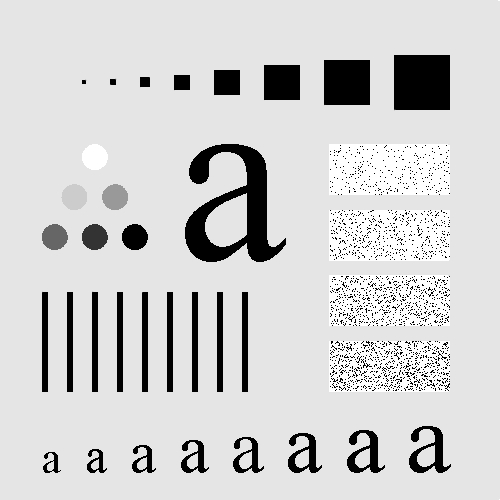
\includegraphics[width=0.5\linewidth]{./images/3/characters.jpg}
        \caption{Original \textit{characters\_test\_pattern.tif}}
        \label{diagram:characters}
    \end{figure}


    \pagebreak
    \subsection{Ideal filter}

        \subsubsection{Low pass}

        \small{\textbf{python problem3.py --ideal -d 5 --low characters\_test\_pattern.tif}}

        \begin{figure}[!htb]\centering
            \begin{minipage}{0.45\textwidth}
                \frame{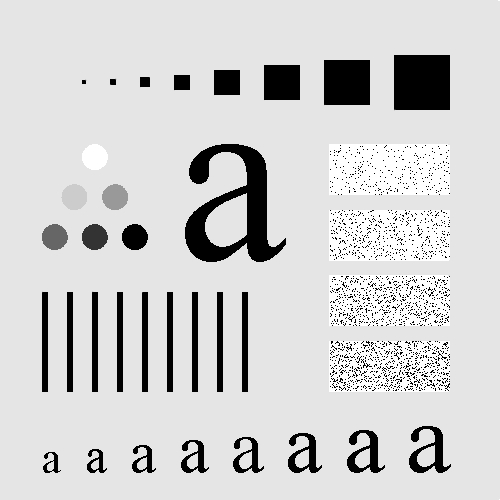
\includegraphics[width=\linewidth]{./images/3/characters.jpg}}
                \caption{Original image}
            \end{minipage}
            \begin{minipage}{0.45\textwidth}
                \frame{
\includegraphics[width=\linewidth]{./images/3/ideal_low_5.jpg}}
                \caption{Ideal low 5}\label{diagram:ideal_low_5}
            \end{minipage}
        \end{figure}

        \begin{figure}[!htb]\centering
            \begin{minipage}{0.45\textwidth}
                \frame{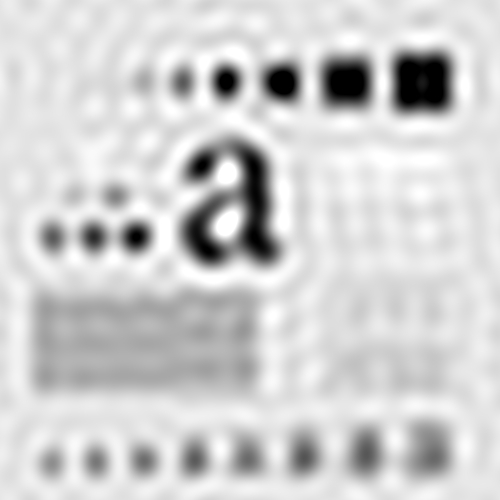
\includegraphics[width=\linewidth]{./images/3/ideal_low_15.jpg}}
                \caption{Ideal low 15}\label{diagram:ideal_low_15}
            \end{minipage}
            \begin{minipage}{0.45\textwidth}
            \frame{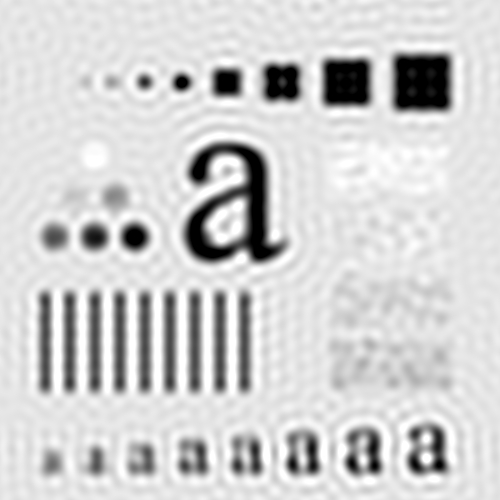
\includegraphics[width=\linewidth]{./images/3/ideal_low_30.jpg}}
            \caption{Ideal low 30}\label{diagram:ideal_low_30}
            \end{minipage}
        \end{figure}

        \pagebreak
        \subsubsection{High pass}

        \small{\textbf{python problem3.py --ideal -d 5 --high characters\_test\_pattern.tif}}

        \begin{figure}[!htb]\centering
            \begin{minipage}{0.45\textwidth}
                \frame{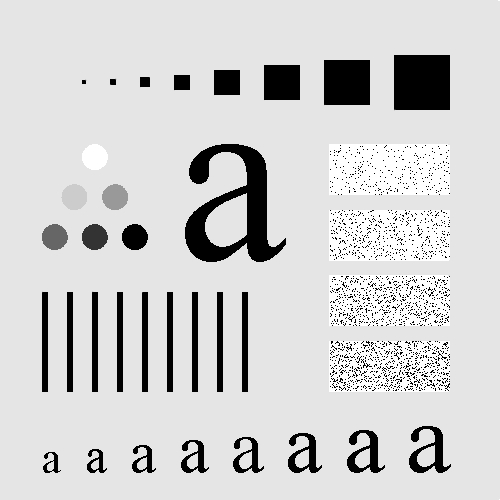
\includegraphics[width=\linewidth]{./images/3/characters.jpg}}
                \caption{\small{Original image}}
            \end{minipage}
            \begin{minipage}{0.45\textwidth}
                \frame{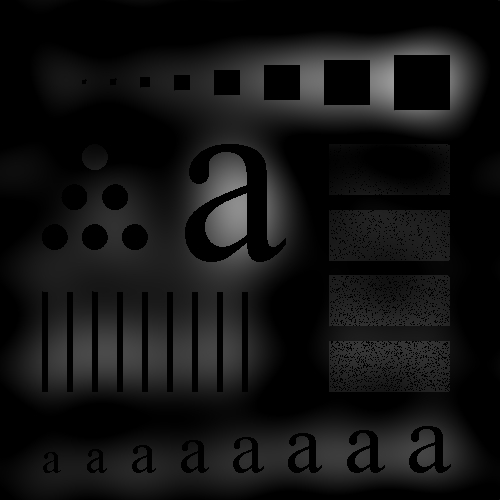
\includegraphics[width=\linewidth]{./images/3/ideal_high_5.jpg}}
                \caption{\small{Ideal high 5}}\label{diagram:ideal_high_5}
            \end{minipage}
        \end{figure}

        \begin{figure}[!htb]\centering
            \begin{minipage}{0.45\textwidth}
                \frame{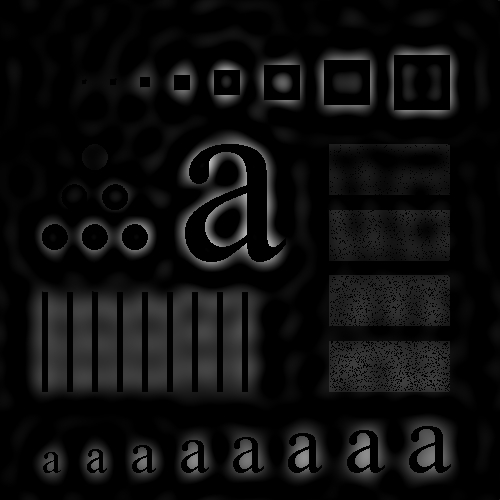
\includegraphics[width=\linewidth]{./images/3/ideal_high_15.jpg}}
                \caption{\small{Ideal high 15}}\label{diagram:ideal_high_15}
            \end{minipage}
            \begin{minipage}{0.45\textwidth}
            \frame{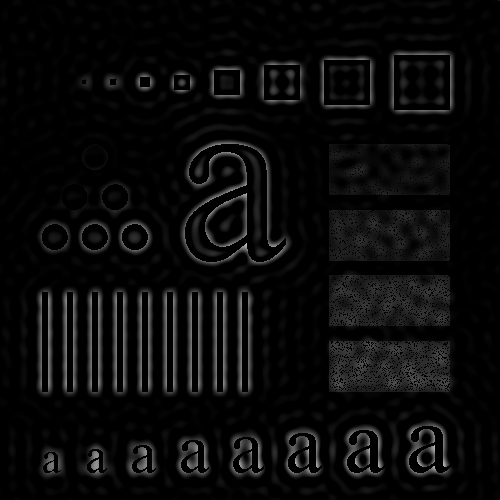
\includegraphics[width=\linewidth]{./images/3/ideal_high_30.jpg}}
            \caption{\small{Ideal high 30}}\label{diagram:ideal_high_30}
            \end{minipage}
        \end{figure}


    \pagebreak
    \subsection{Butterworth order 2 filter}

        \subsubsection{Low pass}

        \small{\textbf{python problem3.py --butterworth -d 5 -n 2 --low characters\_test\_pattern.tif}}

        \begin{figure}[!htb]\centering
            \begin{minipage}{0.45\textwidth}
                \frame{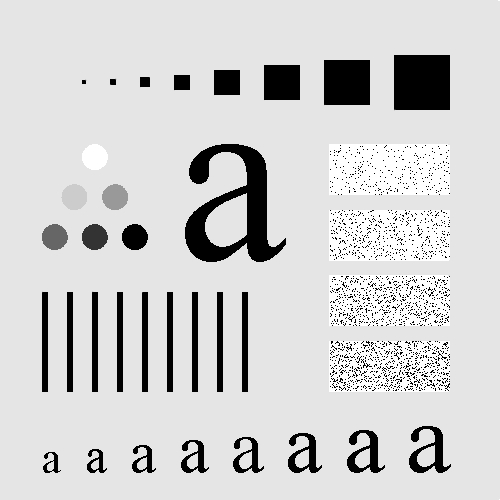
\includegraphics[width=\linewidth]{./images/3/characters.jpg}}
                \caption{\small{Original image}}
            \end{minipage}
            \begin{minipage}{0.45\textwidth}
                \frame{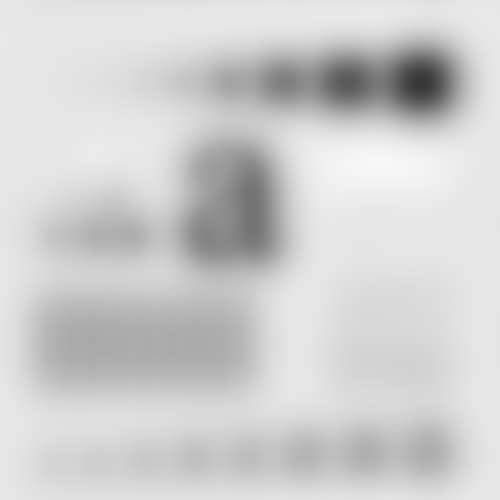
\includegraphics[width=\linewidth]{./images/3/butterworth_low_5_n2.jpg}}
                \caption{\small{Butterworth low 5}}\label{diagram:butterworth_low_5}
            \end{minipage}
        \end{figure}

        \begin{figure}[!htb]\centering
            \begin{minipage}{0.45\textwidth}
                \frame{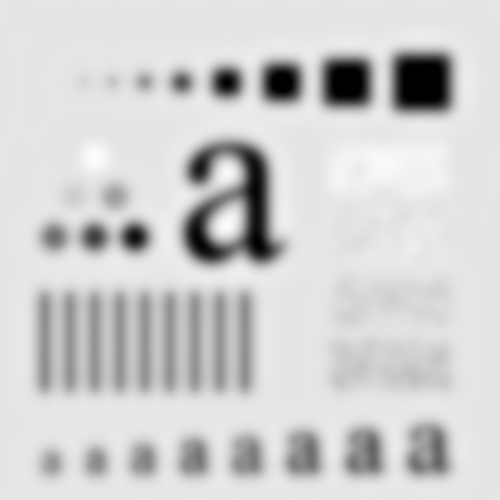
\includegraphics[width=\linewidth]{./images/3/butterworth_low_15_n2.jpg}}
                \caption{\small{Butterworth low 15}}\label{diagram:butterworth_low_15}
            \end{minipage}
            \begin{minipage}{0.45\textwidth}
            \frame{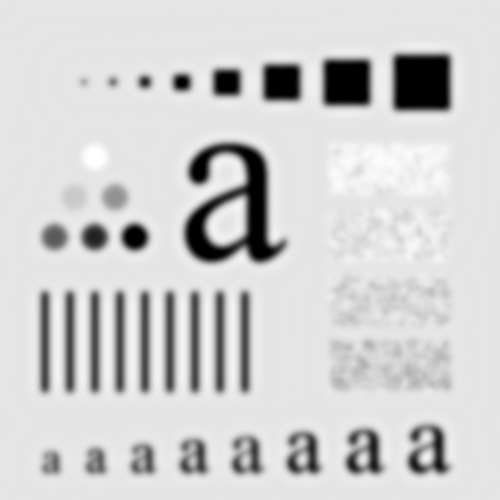
\includegraphics[width=\linewidth]{./images/3/butterworth_low_30_n2.jpg}}
            \caption{\small{Butterworth low 30}}\label{diagram:butterworth_low_30}
            \end{minipage}
        \end{figure}

        \pagebreak
        \subsubsection{High pass}

        \small{\textbf{python problem3.py --butterworth -d 5 -n 2 --high characters\_test\_pattern.tif}}

        \begin{figure}[!htb]\centering
            \begin{minipage}{0.45\textwidth}
                \frame{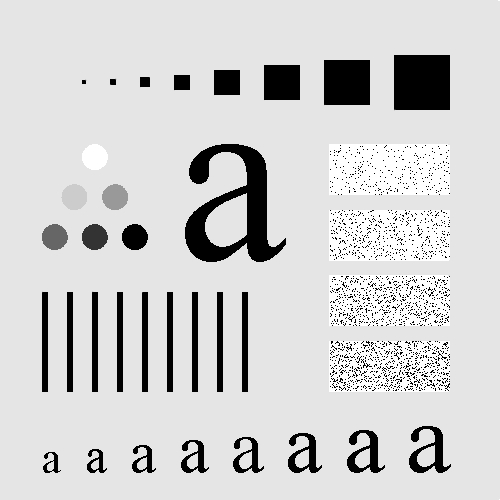
\includegraphics[width=\linewidth]{./images/3/characters.jpg}}
                \caption{\small{Original image}}
            \end{minipage}
            \begin{minipage}{0.45\textwidth}
                \frame{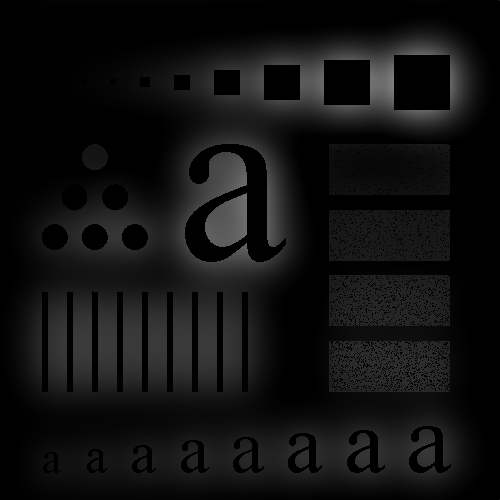
\includegraphics[width=\linewidth]{./images/3/butterworth_high_5_n2.jpg}}
                \caption{\small{Butterworth high 5}}\label{diagram:butterworth_high_5}
            \end{minipage}
        \end{figure}

        \begin{figure}[!htb]\centering
            \begin{minipage}{0.45\textwidth}
                \frame{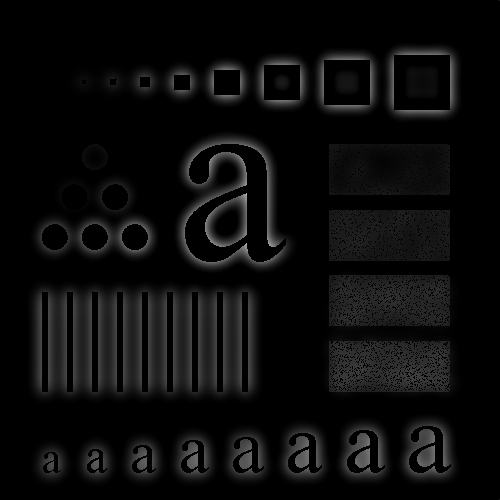
\includegraphics[width=\linewidth]{./images/3/butterworth_high_15_n2.jpg}}
                \caption{\small{Butterworth high 15}}\label{diagram:butterworth_high_15}
            \end{minipage}
            \begin{minipage}{0.45\textwidth}
            \frame{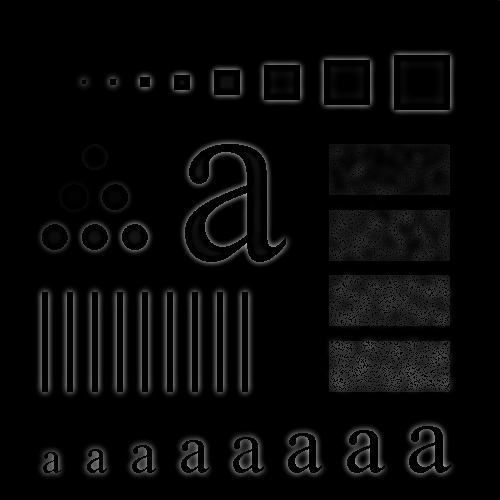
\includegraphics[width=\linewidth]{./images/3/butterworth_high_30_n2.jpg}}
            \caption{\small{Butterworth high 30}}\label{diagram:butterworth_high_30}
            \end{minipage}
        \end{figure}

    \pagebreak
    \subsection{Butterworth order 5 filter}

        \subsubsection{Low pass}

        \small{\textbf{python problem3.py --butterworth -d 5 -n 5 --low characters\_test\_pattern.tif}}

        \begin{figure}[!htb]\centering
            \begin{minipage}{0.45\textwidth}
                \frame{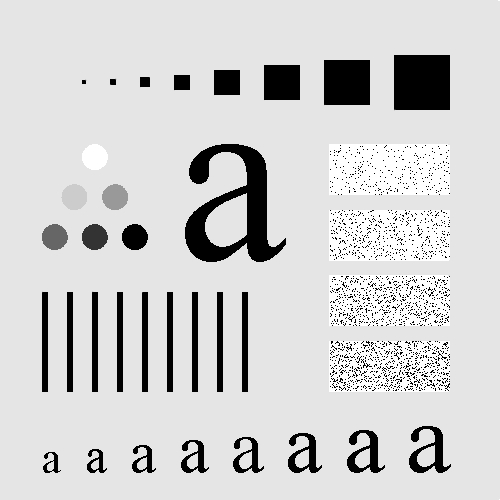
\includegraphics[width=\linewidth]{./images/3/characters.jpg}}
                \caption{\small{Original image}}
            \end{minipage}
            \begin{minipage}{0.45\textwidth}
                \frame{
\includegraphics[width=\linewidth]{./images/3/butterworth_low_5_n5.jpg}}
                \caption{\small{Butterworth low 5}}\label{diagram:butterworth_low_5}
            \end{minipage}
        \end{figure}

        \begin{figure}[!htb]\centering
            \begin{minipage}{0.45\textwidth}
                \frame{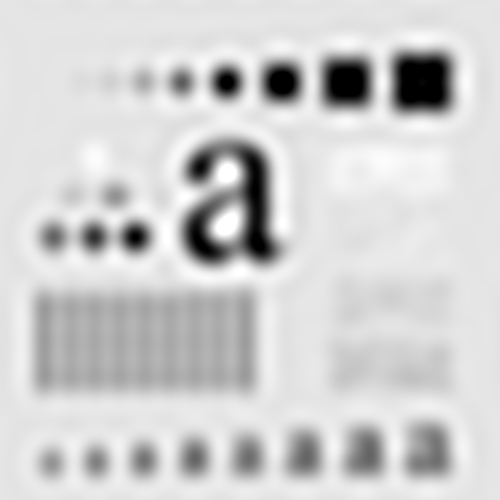
\includegraphics[width=\linewidth]{./images/3/butterworth_low_15_n5.jpg}}
                \caption{\small{Butterworth low 15}}\label{diagram:butterworth_low_15}
            \end{minipage}
            \begin{minipage}{0.45\textwidth}
            \frame{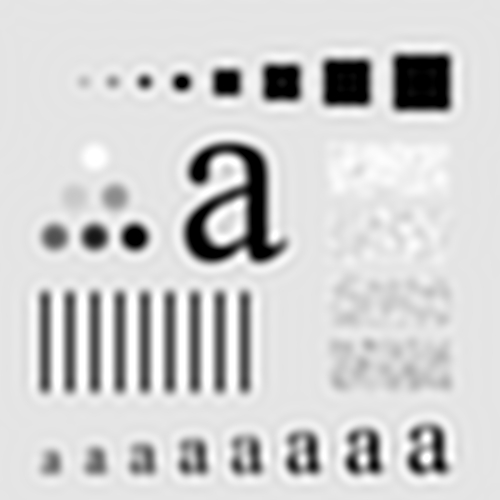
\includegraphics[width=\linewidth]{./images/3/butterworth_low_30_n5.jpg}}
            \caption{\small{Butterworth low 30}}\label{diagram:butterworth_low_30}
            \end{minipage}
        \end{figure}

        \pagebreak
        \subsubsection{High pass}

        \small{\textbf{python problem3.py --butterworth -d 5 -n 5 --high characters\_test\_pattern.tif}}

        \begin{figure}[!htb]\centering
            \begin{minipage}{0.45\textwidth}
                \frame{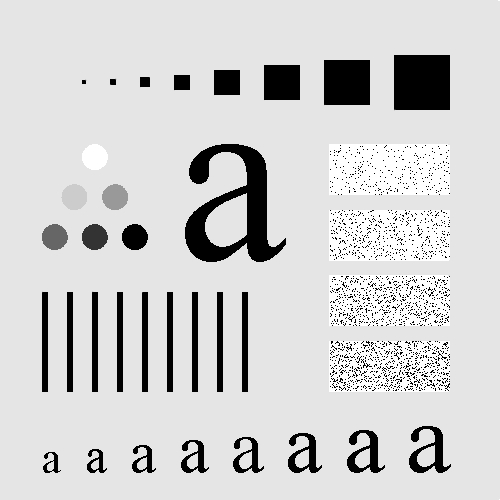
\includegraphics[width=\linewidth]{./images/3/characters.jpg}}
                \caption{\small{Original image}}
            \end{minipage}
            \begin{minipage}{0.45\textwidth}
                \frame{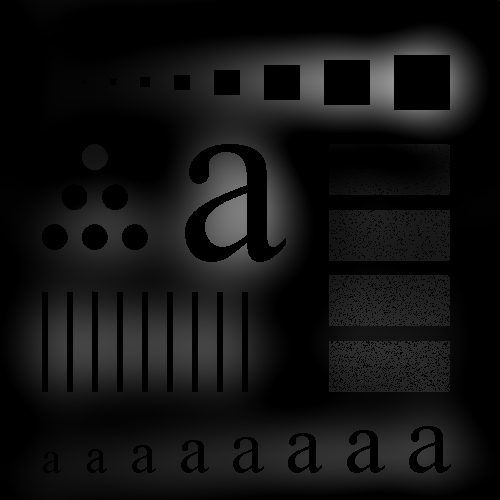
\includegraphics[width=\linewidth]{./images/3/butterworth_high_5_n5.jpg}}
                \caption{\small{Butterworth high 5}}\label{diagram:butterworth_high_5}
            \end{minipage}
        \end{figure}

        \begin{figure}[!htb]\centering
            \begin{minipage}{0.45\textwidth}
                \frame{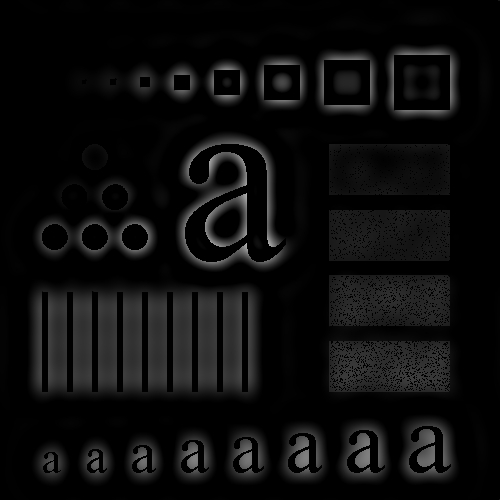
\includegraphics[width=\linewidth]{./images/3/butterworth_high_15_n5.jpg}}
                \caption{\small{Butterworth high 15}}\label{diagram:butterworth_high_15}
            \end{minipage}
            \begin{minipage}{0.45\textwidth}
            \frame{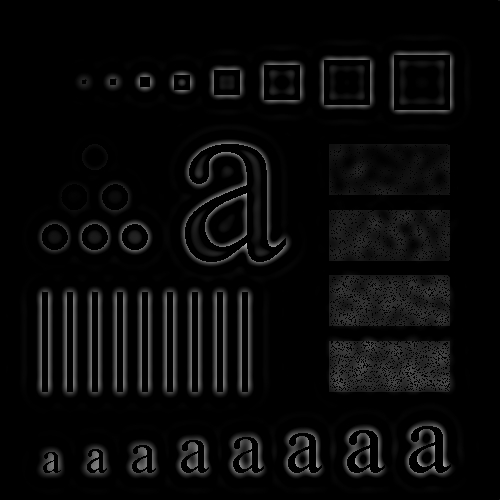
\includegraphics[width=\linewidth]{./images/3/butterworth_high_30_n5.jpg}}
            \caption{\small{Butterworth high 30}}\label{diagram:butterworth_high_30}
            \end{minipage}
        \end{figure}


    \pagebreak
    \subsection{Gaussian filter}

        \subsubsection{Low pass}

        \small{\textbf{python problem3.py --gaussian -d 5 --low characters\_test\_pattern.tif}}

        \begin{figure}[!htb]\centering
            \begin{minipage}{0.45\textwidth}
                \frame{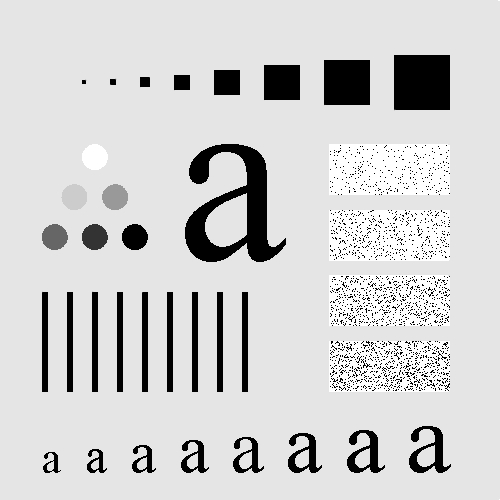
\includegraphics[width=\linewidth]{./images/3/characters.jpg}}
                \caption{Original image}
            \end{minipage}
            \begin{minipage}{0.45\textwidth}
                \frame{
\includegraphics[width=\linewidth]{./images/3/gaussian_low_5.jpg}}
                \caption{Gaussian low 5}\label{diagram:gaussian_low_5}
            \end{minipage}
        \end{figure}

        \begin{figure}[!htb]\centering
            \begin{minipage}{0.45\textwidth}
                \frame{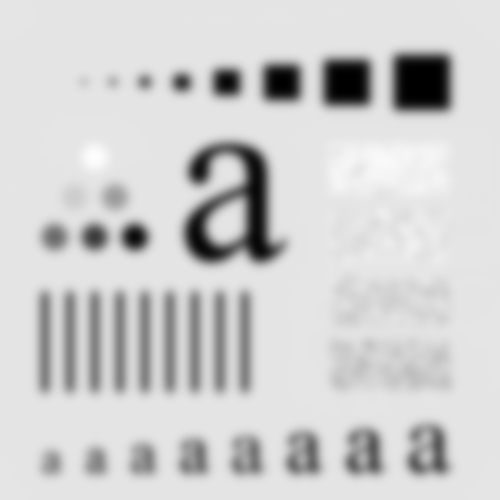
\includegraphics[width=\linewidth]{./images/3/gaussian_low_15.jpg}}
                \caption{Gaussian low 15}\label{diagram:gaussian_low_15}
            \end{minipage}
            \begin{minipage}{0.45\textwidth}
            \frame{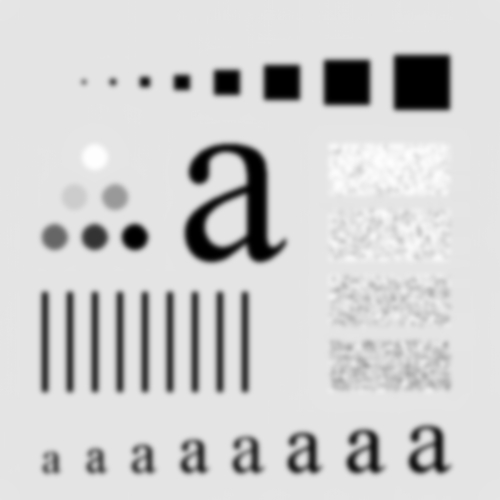
\includegraphics[width=\linewidth]{./images/3/gaussian_low_30.jpg}}
            \caption{Gaussian low 30}\label{diagram:gaussian_low_30}
            \end{minipage}
        \end{figure}

        \pagebreak
        \subsubsection{High pass}

        \small{\textbf{python problem3.py --gaussian -d 5 --high characters\_test\_pattern.tif}}

        \begin{figure}[!htb]\centering
            \begin{minipage}{0.45\textwidth}
                \frame{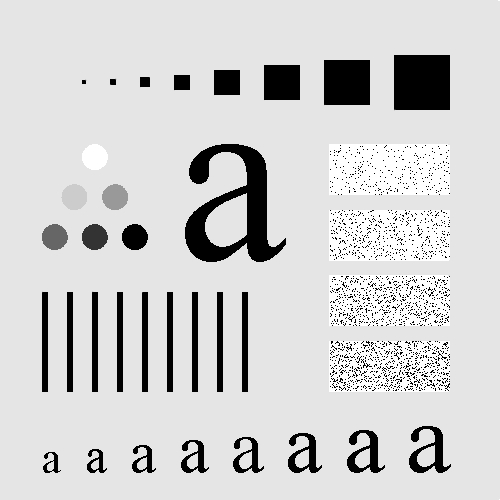
\includegraphics[width=\linewidth]{./images/3/characters.jpg}}
                \caption{\small{Original image}}
            \end{minipage}
            \begin{minipage}{0.45\textwidth}
                \frame{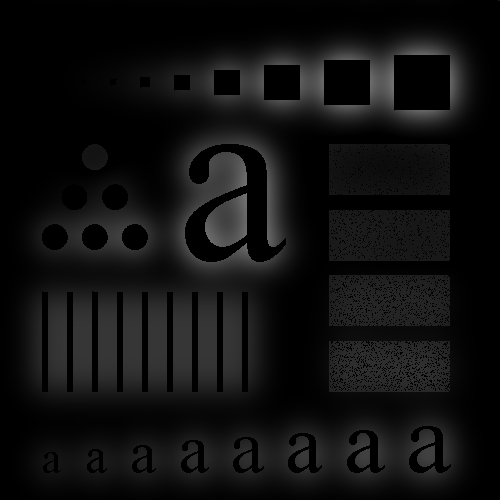
\includegraphics[width=\linewidth]{./images/3/gaussian_high_5.jpg}}
                \caption{\small{Gaussian high 5}}\label{diagram:gaussian_high_5}
            \end{minipage}
        \end{figure}

        \begin{figure}[!htb]\centering
            \begin{minipage}{0.45\textwidth}
                \frame{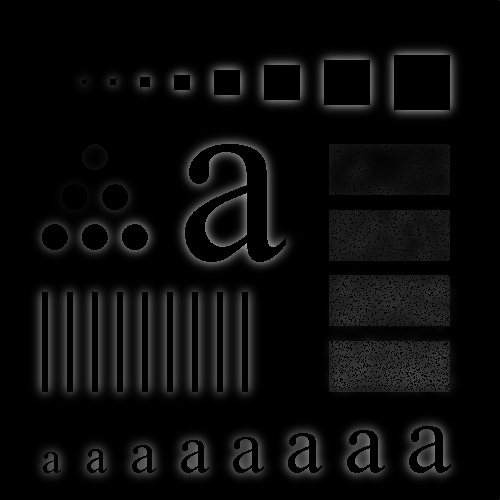
\includegraphics[width=\linewidth]{./images/3/gaussian_high_15.jpg}}
                \caption{\small{Gaussian high 15}}\label{diagram:gaussian_high_15}
            \end{minipage}
            \begin{minipage}{0.45\textwidth}
            \frame{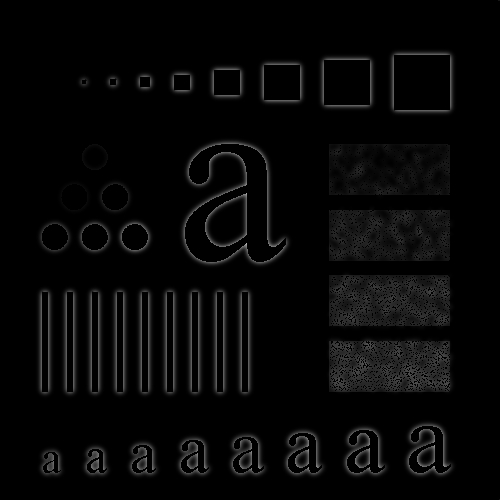
\includegraphics[width=\linewidth]{./images/3/gaussian_high_30.jpg}}
            \caption{\small{Gaussian high 30}}\label{diagram:gaussian_high_30}
            \end{minipage}
        \end{figure}
